\documentclass[a4paper,12pt,french]{book}
\usepackage[margin=2cm]{geometry}
\usepackage{uglix}
\creativecommonsfooter
\begin{document}
\setcounter{chapter}{0}


\chapter{\large Arithmétique\\[-1em]\fontsize{35pt}{42pt}\selectfont\titlefont Bases de numération}
\introduction{Partons sur de bonnes bases.}
 
\begin{definition}[ : ensemble des entiers naturels]
On note $\N$ l'ensemble des \textit{entiers naturels}. $$\N=\lbrace 0;1;2;3;4;5;6;7;8;9;10;11;12\ldots\}$$
\end{definition}

Nous avons l'habitude d'utiliser la base 10 pour représenter les entiers naturels, c'est-à-dire qu'on utilise 10 symboles, appelés \textit{chiffres} 
pour les écrire : 0, 1, 2, \ldots, 9.
Or il n'en a pas toujours été ainsi : 
\begin{enumerate}[--]
	\item 	au \textsc{I}\er millénaire av. J.-C., les Babyloniens utilisaient la base soixante pour mesurer le temps et les angles;
	\item 	durant le \textsc{I}\er millénaire, les Mayas et les Aztèques se servaient de la base vingt (et d'ailleurs en France, 80 se lit \og 
	quatre-vingts\fg);
	\item 	entre le \textsc{vii}\eme et le \textsc{xv}\eme siècle, les astronomes Arabes utilisaient la base cent cinquante pour élaborer des tables 
	permettant de trouver la position d'un astre dans le ciel à un moment donné.
\end{enumerate}
De nos jours, en Informatique, on utilise beaucoup la base deux, dite \textit{binaire} et la base seize, appelée \textit{hexadécimale}.
L'objectif de ce chapitre est de donner les méthodes permettant d'écrire un entier naturel dans une base donnée, plus précisément dans les bases 2, 
10 et 16. Nous verrons également comment passer facilement du binaire à l'hexadécimal et vice-versa.

\section{\'Ecriture binaire d'un entier naturel}
\subsection{Pourquoi le binaire ?}

\double {

Pour simplifier, disons qu'au niveau le plus \og bas \fg{} d'un ordinateur, se trouvent des (millions de) transistors 
qui jouent chacun un rôle d'interrupteur. De multiples points de l'ordinateur peuvent alors être soumis à une tension 
(état 1) ou non (état 0).
En considérant 2 de ces points, on voit que l'état de ce système peut être 00, 01, 10 ou 11. Cela fait 4 possibilités 
et le binaire est né !}
{
\includegraphics[width=4cm]{img/joke1.png}}{4cm}
\subsection{Comprendre l'écriture en base 2}

Puisqu'il n'y a que deux chiffres en binaire, compter est simple mais nécessite rapidement plus de chiffres qu'en base 
10 :\\
\begin{center}
\begin{tabular}{|c|c|c|c|c|c|c|c|c|c|c|}
\hline 
\textbf{\'Ecriture décimale} & 0 & 1 & 2 & 3 & 4 & 5 & 6 & 7 & 8 & \dots\\ 
\hline 
\textbf{\'Ecriture binaire} & 0 & 1 & 10 & 11 & 100 & 101 & 110 & 111 & 1000 &\dots\\ 
\hline 
\end{tabular} \\[1em]
\end{center}

\begin{notation}
On écrira $(11)_{10}$ pour insister sur le fait qu'on parle du nombre 11 \textit{en base 10}, et $(11)_2$ pour dire que c'est une écriture 
binaire.\\
Lorsque ce n'est pas précisé cela veut dire que l'écriture est en base 10.\\
Ainsi $(11)_2=3$ alors que $(11)_{10}$ n'est autre que le 11 \og classique\fg{} et d'ailleurs on le note 11 (sans les parenthèses et le 10 en 
indice).\\
De même, $(111)_2=7$.\\
\end{notation}
Tout entier naturel admet une unique écriture décimale (c'est-à-dire en base 10), il en va de même en binaire:
\begin{propriete}[ : écriture binaire d'un entier naturel]
Tout entier naturel possède une unique écriture en base 2, dite \textit{écriture binaire}.
Plus précisément, soit $n\in\N$, alors il existe un unique entier $k\in\N$ et $k+1$ nombres $a_i$, uniques et valant 0 
ou 1 et tels que $$n=a_02^0+a_12^1+\ldots+a_k2^k$$
ce qui s'écrit aussi $\displaystyle n=\sum_{i=0}^ka_i2^i$.
\end{propriete}

\begin{exemple}
Lorsqu'on regarde le tableau précédent, on voit que $6=(110)_2$.\\Cela s'interprète ainsi :\\

\begin{tabular}{|c|c|c|c|}
	\hline 
	Chiffre binaire & 1 & 1 & 0 \\ 
	\hline 
	Valeur & $2^2$ & $2^1$ & $2^0$ \\ 
	\hline 
\end{tabular}\ \ \ et on obtient un exemple de la propriété précédente : $$6=0\times 2^0+1\times 2^1+1\times 2^2$$
\end{exemple}

\begin{exercice}
	Donner l'écriture décimale des onze premières puissances de deux.
\end{exercice}

\begin{methode}[ 1 : passer de la base 2 à la base 10]
On a un entier écrit en binaire et on veut connaître son écriture en base 10.\\
Par exemple, que vaut $(11101)_2$ ?\\
On fait un tableau dans lequel on met dans la première ligne le nombre en binaire.\\ 
Dans la seconde ligne on indique quelle est la valeur de chaque chiffre binaire.
\begin{center}
	\begin{tabular}{|c|c|c|c|c|c|}
		\hline 
		Chiffre binaire & 1 & 1 & 1 & 0 & 1 \\ 
		\hline 
		Valeur & $2^4$ & $2^3$ & $2^2$ & $2^1$ & $2^0$ \\ 
		\hline 
	\end{tabular}
\end{center}
Ensuite on fait le total :
\begin{tabbing}
		$(11101)_2$	\= 	$=1\times 2^4+1\times 2^3+1\times 2^2+0\times 2^1+1\times 2^0$	\\
			\>	$=16+8+4+1$	\\	
			\>	$=29$	
	\end{tabbing}
Donc $(11101)_2$, c'est 29.
\end{methode}

\begin{exercice}[]
Utiliser la méthode 1 pour déterminer les écritures décimales des nombres suivants
\begin{multicols}{3}
\begin{enumerate}[\bfseries 1.]
	\item 	$(1\,1011)_2$
	\item 	$(11\,0011)_2$
	\item 	$(101\,1011)_2$
	\item 	$(110\,1100)_2$
	\item 	$(1011\,1101)_2$
	\item 	$(10\ 1101\,0011)_2$
\end{enumerate}
\end{multicols}
\end{exercice}
\begin{methode}[ 2 : passer de la base 10 à la base 2]
Ici on veut faire \og dans l'autre sens\fg{} : on a un nombre en base 10 et on veut l'écrire en binaire.\\
Commençons par nous rappeler comment on fait avec une écriture décimale :
			\begin{tabbing}
				243	\= 	$=2\times 100+4\times 10 +3$	\\
				
					\>	$=2\times 10^2+4\times 10^1+3\times 10^0$
			\end{tabbing}
En fait, on a trouvé tout seul que 243 commence par s'écrire avec des \textit{centaines} (plus précisément 2 centaines).
Une fois qu'on a compté ces deux centaines, il reste 43 et on recommence : il faut 4 dizaines, et 3 unités.\\


On peut faire la même chose en base 2 : on commence par repérer quelle est la plus grande puissance de 2 inférieure à 243 : c'est 128.
			\begin{tabbing}
				243	\= 	$=128+115\qquad$ on recommence avec 115\\
				
				
					\>	$=128+64+51\qquad$ on continue avec 51\\
					
					\>	$=128+64+32+19\qquad$ puis avec 19	\\
					
					\>	$=128+64+32+16+3\qquad$ puis avec 3	\\
							
					\>	$=128+64+32+16+2+1\qquad$ c'est terminé	\\
														
					\> $=2^7+2^6+2^5+2^4+2^1+2^0\qquad0$ il n'y a plus qu'à écrire en binaire\\
					
					\> $=(11110011)_2$
			\end{tabbing}
			Cette méthode est pratique quand l'entier est petit et que l'on connaît bien les premières puissances de deux.\\
			Quand ce n'est pas le cas, une autre méthode (la méthode 3) peut être employée.	
\end{methode}

\begin{exercice}[]
	Utiliser la méthode 2 pour déterminer les écritures binaires des nombres suivants
	\begin{multicols}{3}
		\begin{enumerate}[\bfseries 1.]
			\item 	17
			\item 	36
			\item 	130
			\item 	192
			\item	231
			\item 	1283
		\end{enumerate}
	\end{multicols}
\end{exercice}
\subsection{L'algorithme des divisions successives}

C'est un algorithme très important car il est valable en base 10, en base 2 et aussi en base 16 (que nous verrons plus tard)

\begin{definition}[ : division euclidienne dans \N]

Soient A et B deux entiers naturels, et $B\neq 0$. Il existe deux nombres uniques Q et R (vérifiant $0\geqslant R<B$) tels que l'on puisse écrire
$$A = Q\times B + R$$

C'est exactement la division que l'on a apprise en sixième (celle où l'on s'arrête aux nombres entiers):
\begin{center}
\begin{tabular}{r|l}
A & B\\
\cline{2-2}
R & Q
\end{tabular}

\begin{enumerate}[\textbullet]
	\item 	A est appelé le \textit{dividende};
	\item 	B est le \textit{diviseur};
	\item	Q est le \textit{quotient};
	\item 	R est le \textit{reste}, il est \textit{impérativement} plus petit que B.
\end{enumerate}
\end{center}
\end{definition}
\begin{methode}[ 3]
On va retrouver les chiffres de 243 en base 10 en faisant des divisions successives par 10. On sait déjà que ce sont 2,4 et 3 mais c'est un exemple 
pour comprendre comment cela marche et pour passer à la base 2 ensuite.\\
On divise 243 par 10 en faisant une division euclidienne : 
\begin{center}
\begin{tabular}{r|l}
243&10\\
\cline{2-2}
\boxed{3} &24\\
\end{tabular}
\hspace{1cm}$243 = 24\times 10 + \boxed{3}$
\end{center}

Comme le quotient (24) n'est pas nul, on recommence, jusqu'à ce que le quotient soit nul :

\begin{center}
\begin{tabular}{r|l}
24&10\\
\cline{2-2}
\boxed{4} &2\\
\end{tabular}
\hspace{1cm}$24 = 2\times 10 + \boxed{4}$
\hspace{1cm}
\begin{tabular}{r|l}
2&10\\
\cline{2-2}
\boxed{2} &0\\
\end{tabular}
\hspace{1cm}$2 = 0\times 10 + \boxed{2}$
\end{center}

Quand on trouve un quotient nul, on reprend tous les restes à l'envers :2, 4 et 4, cela nous donne 243.\\

En fait, il est plus pratique d'enchainer les divisions comme ceci :
$$\division[10]{243}$$

Pour trouver l'écriture binaire, de 243 on fait pareil mais avec des divisions par 2 :


$$\division{243}$$

Dès qu'on a trouvé un quotient nul on remet les restes dans l'ordre inverse : $$243 = (11110011)_2$$
\end{methode}

\begin{remarque}[]
Attention à bien écrire les restes \textit{dans l'ordre inverse} de celui dans lequel ils apparaissent.
\end{remarque}

\begin{exercice}[]
	Utiliser la méthode 3 pour déterminer les écritures binaires des nombres suivants
	\begin{multicols}{3}
		\begin{enumerate}[\bfseries 1.]
			\item 	12
			\item 	37
			\item 	69
			\item 	145
			\item	251
			\item 	1234
		\end{enumerate}
	\end{multicols}
\end{exercice}
\subsection{Vocabulaire lié à l'informatique}

\begin{enumerate}[--]
\item 	Un chiffre décimal peut être 0, 1, 2, 3, 4, 5, 6, 7, 8 ou 9.\\
		Un chiffre binaire peut être seulement 0 ou 1. En Anglais, \textit{chiffre binaire} se traduit par \textit{binary digit}, 
		que l'on abrège en \textit{bit}. On garde cette dénomination en Français.\\
		Le bit est donc \og le plus petit morceau d'information numérique \fg{}.
\item 	On regroupe les chiffres décimaux par paquets de 3, comme dans 1 230 014 par exemple.
		En binaire on groupe les bits par 4.\\
		Bien souvent les bits sont groupés par 8 (deux paquets de 4). Un tel paquet s'appelle un \textit{octet}.
\item 	Lorsqu'on considère un nombre écrit en binaire, on parle souvent de \textit{bit de poids fort} et de 
\textit{bit de poids faible} pour parler respectivement du bit associé à la plus grande puissance de 2, et du bit 
d'unités.\\
		Considérons $(0010\ 0101)_2$. Son bit de poids fort est 0, son bit de poids faible est 1.
\end{enumerate}

\begin{exercice}[]
\begin{enumerate}[\bfseries 1.]
	\item 	Que peut-on dire d'un entier dont le bit de poids faible de son écriture binaire vaut 0 ? Pourquoi ?
	\item 	Même question pour un entier dont les 2 bits de poids les plus faibles de son écriture binaire valent 0.
\end{enumerate}
\end{exercice}

\begin{exercice}[]
	\begin{enumerate}[\bfseries 1.]
		\item 		Si on décide, en machine, de représenter des entiers naturels par leur écriture binaire sur 4 bits, combien pourra-t-on en représenter ? Quels seront les plus petit et le plus grand nombre représentables ?
		\item 	Même question, mais en écrivant les entiers sur $n$ bits, où $n$ est un entier positif.
	\end{enumerate}
\end{exercice}
\section{\'Ecriture hexadécimale d'un entier naturel}

La base \og naturelle \fg{} de l'informatique est la base 2, mais elle n'est pas très pratique car elle donne lieu à 
des écritures trop longues.
La base 10 nous paraît bien meilleure parce que nous avons l'habitude de l'utiliser, mais elle ne fait pas bon ménage 
avec la base 2 : il n'y a pas de méthode simple pour passer du décimal au binaire, et vice versa.\\
La base 16, ou base \textit{hexadécimale}, est en revanche très adaptée à l'écriture des paquets de 4 bits, et par 
extension à celle des octets et autres écritures binaires.\\

En hexadécimal, on dispose de 16 chiffres : 0, 1, 2, 3, 4, 5, 6, 7, 8, 9, A, B, C, D, E et F.

\begin{propriete}[ : écriture binaire d'un entier naturel]
Tout entier naturel possède une unique écriture en base 16, dite \textit{écriture hexadécimale}.
Plus précisément, soit $n\in\N$, alors il existe un unique entier $k\in\N$ et $k+1$ nombres $a_i$, uniques et valant 0, 1, 2, \ldots, ou F et tels 
que $$n=a_016^0+a_16^1+\ldots+a_k16^k$$
ce qui s'écrit aussi
 $$n=\sum_{i=0}^ka_i16^i$$
\end{propriete}

\begin{remarque}
On a vu une propriété similaire en base 2 et en fait elle est valable \textit{dans toutes les bases}  $b$ (où $b$ est un entier naturel supérieur ou 
égal à 2). Cela justifierait par exemple l'utilisation de la base 20 ou de la base 150.
\end{remarque}

Les méthodes que l'on a vues en base 2 et 10 se transposent en base 16.
\begin{methode}[ 4 : passer de la base 16 à la base 10]
Déterminons l'écriture décimale de $(D4A)_{16}$.\\ Il faut garder en tête les valeurs suivantes :
\begin{center}
\begin{tabular}{|l|c|c|c|c|c|c|}
\hline 
chiffre hexadécimal & A & B & C & D & E & F \\ 
\hline 
valeur  & 10 & 11 & 12 & 13 & 14 & 15 \\ 
\hline 
\end{tabular} 
\end{center}
Ainsi, si l'on veut l'écriture décimale de 	$(D4A)_{16}$ , on écrit :
\begin{tabbing}
	$(D4A)_{16}$  	\= $=13\times 16^2 + 4\times 6 + 10\times 16^0$	 car D vaut 13 et A vaut 10.\\
		\>	$=3402$
\end{tabbing}
\end{methode}

\begin{exercice}[]
	Utiliser la méthode 4 pour déterminer les écritures décimales des nombres suivants
	\begin{multicols}{3}
		\begin{enumerate}[\bfseries 1.]
			\item 	$(12)_{16}$
			\item 	$(2A)_{16}$
			\item 	$(F2)_{16}$
			\item 	$(100)_{16}$
			\item	$(88)_{16}$
			\item 	$(3E2)_{16}$
		\end{enumerate}
	\end{multicols}
\end{exercice}
\begin{methode}[ 5 : passer de la base 10 à la base 16]
Déterminons maintenant l'écriture hexadécimale de 503: on fait des divisions successives par 16 tout comme en base 2
$$\division[16]{503}$$
On s'arrête car on a trouvé un quotient nul et on remet les restes dans l'ordre inverse : 1, 15, 7 cela fait 1, F et 7 : $503=(1F7)_{16}$.
\end{methode}
\begin{exercice}[]
	Utiliser la méthode 5 pour déterminer les écritures hexadécimales des nombres suivants
	\begin{multicols}{3}
		\begin{enumerate}[\bfseries 1.]
			\item 	29
			\item 	50
			\item 	123
			\item 	487
			\item	510
			\item 	2020
		\end{enumerate}
	\end{multicols}
\end{exercice}

\begin{center}
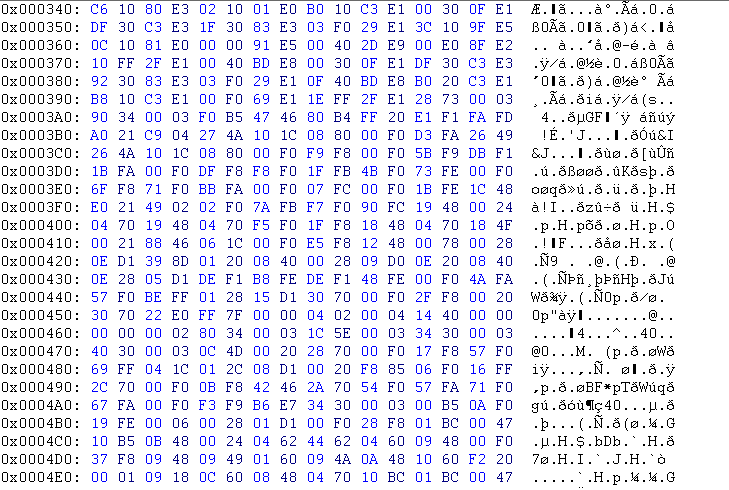
\includegraphics[width=11cm]{img/hex.png}\\
\textit{\small Un éditeur hexadécimal montre le contenu d'un fichier, d'un disque dur, ou de la RAM d'un ordinateur. La première colonne indique l'adresse, 
puis 16 octets écrits en hexadécimal et enfin les caractères correspondants.}
\end{center}

\begin{center}
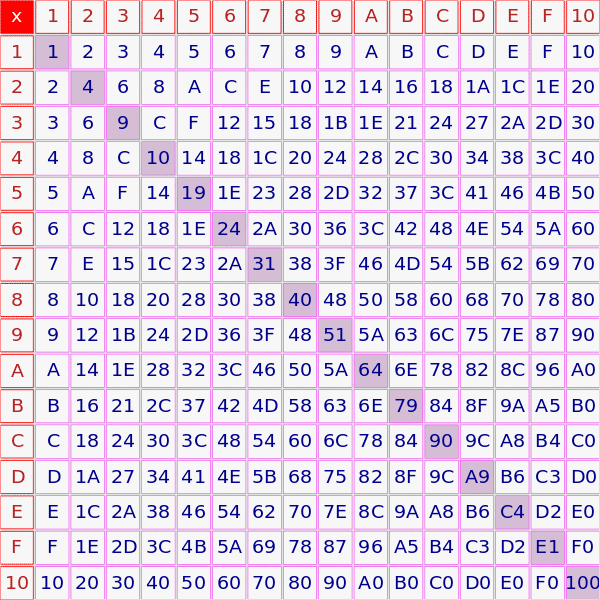
\includegraphics[width=12cm]{img/hexmult.png}\\
\textit{\small Table de multiplication hexadécimale.}
\end{center}
\section{Hexadécimal et binaire : un mariage heureux}
En fait il est très simple de passer d'une écriture en base 2 à une écriture en base 16 et vice-versa. On utilise le tableau suivant :
\begin{center}
\begin{tabular}{|c|c|c|c|c|c|c|c|c|}
\hline 
\rowcolor{orange@color!15}
Base 16 & 0 & 1 & 2 & 3 & 4 & 5 & 6 & 7 \\
\hline 
Base 2 & 0000 & 0001 & 0010 & 0011 & 0100 & 0101 & 0110 & 0111  \\ 
\hline 
\rowcolor{orange@color!15}
Base 16 & 8 & 9 & A & C & B & D & E & F \\ 
\hline
Base 2 & 1000 & 1001 & 1010 & 1011 & 1100 & 1101 & 1110 & 1111\\
\hline
\end{tabular} 
\end{center}
Ensuite on peut utiliser ce tableau dans les 2 sens :
\begin{methode}[ 6 : passer de la base 2 à la base 16]
\begin{tabbing}
	$(101101000011101)_2$	\=	$=(0101\ 1010\ 0001\ 1101)_2$\\
				\>	$=\left(\underbrace{0101}_5\ \underbrace{1010}_A\ \underbrace{0001}_1\ \underbrace{1101}_D\right)_2$\\
				\>	$=(5A1D)_{16}$
\end{tabbing}
\end{methode}
\begin{exercice}[]
	En utilisant la méthode 6,  déterminer les écritures hexadécimales des nombres suivants
		\begin{multicols}{2}
			\begin{enumerate}[\bfseries 1.]
				\item 	$(1010\,1111)_2$
				\item 	$(10\,1011)_2$
				\item 	$(1110\,1000)_2$
				\item 	$(1\,1010\,1111)_2$
			\end{enumerate}
		\end{multicols}
\end{exercice}
\begin{methode}[ 7 : passer de la base 16 à la base 2]
\begin{tabbing}
$(F7B)_{16}$\=$=\left(\underbrace{1111}_F\ \underbrace{0111}_7\ \underbrace{1101}_B\right)_2$\\
			\>$=\left(1111\,0111\,1101\right)_2$
\end{tabbing}
\end{methode}
\begin{exercice}[]
	En utilisant la méthode 7,  déterminer les écritures binaires des nombres suivants
	\begin{multicols}{2}
		\begin{enumerate}[\bfseries 1.]
			\item 	$(FF)_{16}$
			\item 	$(A2)_{16}$
			\item 	$(3D)_{16}$
			\item 	$(7E8)_{16}$
		\end{enumerate}
	\end{multicols}
\end{exercice}

\exostart




\begin{exercice}
\begin{enumerate}[\bfseries 1.]
	\item 	Calculer $2^6+2^4+2^3+2^0$.
	\item 	En déduire l'écriture binaire de 89.	
\end{enumerate}
\end{exercice}


\begin{exercice}
\begin{enumerate}[\bfseries 1.]
	\item 	Calculer $2^7+2^3+2^2+2^1$.
	\item 	En déduire l'écriture décimale de  $(1000 1110)_2$.	
\end{enumerate}
\end{exercice}


\begin{exercice}[]
En utilisant la méthode 2, donner l'écriture binaire de 
\begin{enumerate}[\bfseries 1.]
	\item 	56
	\item 	35
	\item 	13	
\end{enumerate}
\end{exercice}

\begin{exercice}[]
En utilisant la méthode 3, donner l'écriture binaire de 
\begin{enumerate}[\bfseries 1.]
	\item 	142
	\item 	273
	\item 	1000
\end{enumerate}
\end{exercice}

\begin{exercice}
\begin{enumerate}[--]
		\item 	Donner l'écriture décimale de $(1101\ 1010)_2$.
		\item 	Donner l'écriture binaire de 2016.
		\item 	Donner l'écriture hexadécimale de 2016.
\end{enumerate}
\end{exercice}

\begin{exercice}
\begin{enumerate}[--]
		\item 	Donner les écritures décimales de $(11)_2$, $(111)_2$, $(1111)_2$.
		\item   Soit $n \in \N$, conjecturer (c'est-à-dire faire une hypothèse sur) la valeur de $ \left(\underbrace{1\ldots 1}_{n \textrm{ chiffres}}\right)_2$.
\end{enumerate}
\end{exercice}


\begin{exercice}
Pour multiplier par dix un entier naturel exprimé en base dix, il suffit d'ajouter un 0 à sa
droite, par exemple, $12\times 10 = 120$.\\
Quelle est l'opération équivalente pour les entiers naturels exprimés en base deux ?
\end{exercice}

\begin{exercice}[]
	Le code \textsl{ASCII} (\textit{American Standard Code for Information Interchange}) permettait de coder les caractères principaux utilisés en Informatique. 
	De nos jours on lui préfère l'UTF-8, mais ce dernier est rétro-compatible.
	\begin{center}
		\includegraphics[width=16cm]{img/ASCII.png}	
	\end{center}
	\begin{enumerate}[\bfseries 1.]
		\item 	Donner le code du caractère \og F\fg{} en binaire.
		\item 	Combien faudrait-il de \textit{bits} pour représenter un caractère de cette table ?
		\item 	En pratique, on code sur un \textit{octet}, c'est à dire 8 \textit{bits}.\\
		Quelle suite d'octets (en hexadécimal) correspond au mot \og Fred\fg{} ?
		\item 	Quelle opération arithmétique permet de passer d'un caractère majuscule au caractère minuscule correspondant ? Donner un exemple.\\
		Et dans l'autre sens ?
		\newpage
		\item  	On utilise un éditeur hexadécimal, voici ce que l'on voit :
		\begin{center}
			\includegraphics[width=16cm]{img/editeur.png}
		\end{center}
		
		Retrouver le contenu de la variable de type chaîne de caractères de longueur 6 encodée en \textsc{ASCII} qui est stockée à partir de l'adresse $(0001\ 1011\ 1101\ 0101\ 0000\ 0001\ 0010\ 1100)_2$	
	\end{enumerate}
\end{exercice}
\creativecommonsheader
\end{document}
